%% Submissions for peer-review must enable line-numbering
%% using the lineno option in the \documentclass command.
%%
%% Preprints and camera-ready submissions do not need
%% line numbers, and should have this option removed.
%%
%% Please note that the line numbering option requires
%% version 1.1 or newer of the wlpeerj.cls file, and
%% the corresponding author info requires v1.2

\documentclass[fleqn,10pt,lineno]{wlpeerj} % for journal submissions

% ZNK -- Adding headers for pandoc

\setlength{\emergencystretch}{3em}
\providecommand{\tightlist}{
\setlength{\itemsep}{0pt}\setlength{\parskip}{0pt}}
\usepackage{lipsum}
\usepackage[unicode=true]{hyperref}
\usepackage{longtable}



\usepackage{lipsum}

\title{Combining data, distribution summary, model effects, and uncertainty in
a single plot}

\author[\href{mailto:walker@maine.edu}{\nolinkurl{walker@maine.edu}}]{Jeffrey A. Walker}




%
% \author[1]{First Author}
% \author[2]{Second Author}
% \affil[1]{Address of first author}
% \affil[2]{Address of second author}
% \corrauthor[1]{First Author}{f.author@email.com}

% 

\begin{abstract}

% Dummy abstract text. Dummy abstract text. Dummy abstract text. Dummy abstract text. Dummy abstract text. Dummy abstract text. Dummy abstract text. Dummy abstract text. Dummy abstract text. Dummy abstract text. Dummy abstract text.
\end{abstract}

\usepackage{amsthm}
\newtheorem{theorem}{Theorem}[section]
\newtheorem{lemma}{Lemma}[section]
\theoremstyle{definition}
\newtheorem{definition}{Definition}[section]
\newtheorem{corollary}{Corollary}[section]
\newtheorem{proposition}{Proposition}[section]
\theoremstyle{definition}
\newtheorem{example}{Example}[section]
\theoremstyle{definition}
\newtheorem{exercise}{Exercise}[section]
\theoremstyle{remark}
\newtheorem*{remark}{Remark}
\newtheorem*{solution}{Solution}
\begin{document}

\flushbottom
\maketitle
\thispagestyle{empty}

\section*{Introduction}\label{introduction}
\addcontentsline{toc}{section}{Introduction}

Recommended best practices for the reporting of statistical results
include 1) showing the raw data and/or distribution of data in plots
(Drummond and Vowler 2011; Tracey L. Weissgerber et al. 2015; M. Spitzer
et al. 2014; Krzywinski and Altman 2014; Harrell 2014; Tracey L
Weissgerber et al. 2016) and focusing on 2) effect size and (3)
uncertainty in effect estimates instead of \(p\)-values of null
hypothesis tests (Nakagawa and Cuthill 2007; Yoccoz 1991; Johnson 1999;
Curran-Everett, Taylor, and Kafadar 1998). By contrast, standard
practice throughout experimental biology includes the reporting of ANOVA
results in tables and treatment means and standard errors of the mean in
plots. At best, ANOVA tables poorly communicate effect size and
uncertainty. Effects and uncertainty can be inferred from plots of
treatment means and standard errors only indirectly.

Here, I introduce the Harrell plot, a tool to communicate statistical
results from experiments, or any analysis with categorical independent
variables (ANOVA-like linear models). A Harrell plot combines 1) a dot
plot to show individual values, 2) a box plot to show the distribution
of the response within treatment groups, and 3) a forest plot of effect
estimates and confidence intervals to show modeled effect sizes and
uncertainty. The combination of the effects in the top part and
distribution in the bottom part of a Harrell plot was inspired by Fig.
1.1 of Harrell (2014). The Harrell plot is implemented both as an online
HarrellPlot Shiny app for users with no or limited R experience,
including undergraduate biology majors, and the R package HarrellPlot,
for users with some R experience.

\section*{Effect size and
uncertainty}\label{effect-size-and-uncertainty}
\addcontentsline{toc}{section}{Effect size and uncertainty}

By effect, or effect size, I mean the magnitude and direction of the
difference in response to some treatment, or some combination of
treatments. If the mean critical thermal minimum is 5.1 \(^\circ\) C in
the control group of flies and 5.8 \(^\circ\) C in the treated group,
then the effect is
\(5.8 ^\circ \textrm{C} - 5.1 \textrm{C} = +0.7 ^\circ \textrm{C}\). The
non-intercept coefficients of a linear model are effects. Contrasts of a
linear model are effects. A confidence interval of the effect is a
measure of the uncertainty in the estimate. A 95\% confidence interval
of the effect has a 95\% probability (in the sense of long-run
frequency) of containing the true effect. This probability is a property
of the population of intervals that could be computed using the same
sampling and measuring procedure. It is not correct, without further
assumptions, to state that there is a 95\% probability that the true
effect lies within the interval. However, if we have only weak prior
beliefs about the possible values of the effect, then it is valid,
though possibly misleading, to state that there is an approximately 95\%
probability that the true effect lies in the interval (Greenland and
Poole 2013; Gelman 2013). Perhaps a more useful interpretation is that
the interval contains the range of effects that are consistent with the
data, in the sense that a \(t\)-test would not reject the null
hypothesis of a difference between the estimate and any value within the
interval (this interpretation does not imply anything about the true
value).

While many experiments in biology are conducted with a proximate goal of
discovering or confirming that an effect exists (that is, the effect is
something other than zero), the ultimate goal of a research program
should be to understand the biological (including clinical, behavioral,
ecological or evolutionary) consequences of effects (Yoccoz 1991;
Curran-Everett, Taylor, and Kafadar 1998; Nakagawa and Cuthill 2007;
Batterham and Hopkins 2006). These consequences are functions of effect
magnitude and direction and, consequently, estimates of effect size and
uncertainty are tools for these ultimate goals. By contrast, hypothesis
testing and \(p\)-values are tools only for the more proximate goal of
effect presence. Importantly, the discovery that an effect exists
requires more than a \(p\)-value, including both replicate experiments
and modified experiments that ``probe their experimental systems in
multiple, independent ways'' (Vaux 2012; see also Munafò and Davey Smith
2018). Probing is standard in much of cell and molecular biology (but
see Kaelin Jr 2017). Replications are uncommon throughout most of
experimental biology. It probably cannot be emphasized enough that
finding statistically significant \(p\)-values is a very low-bar in
experimental biology. All components of complex physiological systems
are causally connected and perturbing any feature of a system will have
some effect on everything, however small (this may not be true in a
simplified experimental system with a minimal number of components).
Consequently, Type I errors will not exist in complex systems and the
concept of null-hypothesis testing becomes meaningless. Instead,
researchers should be concerned with sign and magnitude errors
{[}Gelman\_Power\_2014{]} and with conditional dependencies.

\begin{figure}
\includegraphics[width=1\linewidth]{harrell_plot_intro_files/figure-latex/confidence-1} \caption{Magnitude based inference using confidence intervals}\label{fig:confidence}
\end{figure}

Confidence intervals of effects can be (and are most often) used to
infer ``statistical significance''. Statisticians have long advocated
for the far more valuable use of a confidence interval as a tool to
infer the sensitivity of an interpretation or conclusion to the data
(Tukey 1991). Again, a confidence interval of an effect gives the range
of parameter values that are consistent with the data (Amrhein,
Korner-Nievergelt, and Roth 2017). Consequently, as evidence for a
theory in academic biology or a decision in applied biology, the whole
range of values within a confidence interval, and not just the mean or
median, should be consistent with an interpretation or conclusion,
otherwise the data are ambiguous (or ``inconclusive'', but this might
suggest that the results from a single study could ever be
``conclusive''). One scheme for implementing this strategy is
``magnitude-based inference'', summarized in figure
\ref{fig:confidence}, which is a modification of figure 2 of (Barker and
Schofield 2008), which itself is a corrected interpretation of figure 2
in (Batterham and Hopkins 2006) (of course, by merely creating a
boundary between trivial and consequential effect size, this strategy
encourages rather than discourages dichotomization).

\begin{figure}
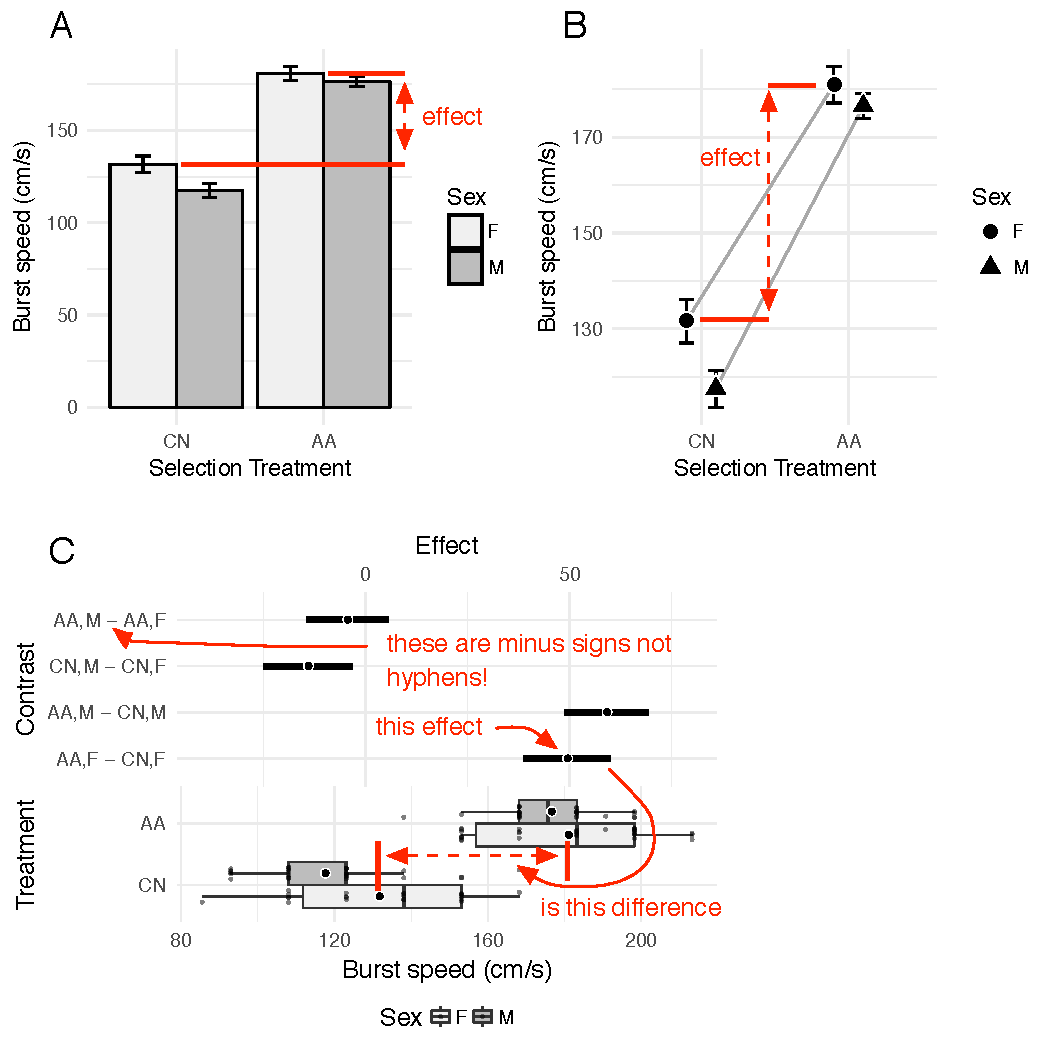
\includegraphics[width=1\linewidth]{../figs/fig1} \caption{Three methods for communicating results of an experiment. In the bar plot (A) and a Cleveland dot plot (B), the treatment effect is inferred by mentally computing the distance between treatment means. In the Harrell plot (C), the treatment effect is plotted in addition to the treatment means. Key: AA selected flies, CN control flies, F female, M male}\label{fig:plots}
\end{figure}

\subsection*{Mean-and-error plots}\label{mean-and-error-plots}
\addcontentsline{toc}{subsection}{Mean-and-error plots}

Figure \ref{fig:plots}A and B illustrate two kinds of mean-and-error
plot. The unpublished data are the maximum burst speed of
\emph{Drosophila melanogaster} individuals from two lines that have
undergone selection in a compartmentalized wind tunnel (weber, marden
xxx) and two control lines. Maximum burst speed was measured on
individual flies that were stimulated to take-off and fly against a wind
of known speed in a wind tunnel. The mean response of a group is
represented either by the height of the bar (A) or a point symbol (B).
The error bar most commonly represents one standard error of the mean; a
confidence interval is less common. Occasionally, the error bar
represents one sample standard deviation. Bar-and-error plots are
ubiquitous in experimental cell biology. Point-and-error plots are more
common in animal physiology than in cell biology. Perhaps because of the
ubiquity of bar plots in cell biology (including the pages of Science,
Nature, and Cell), most criticism of mean-and-error plots focusses on
bar plots, which are pejoratively called ``dynamite'', ``plunger'', or
``antenna'' plots.

Three, related criticisms of mean-and-error plots are (Drummond and
Vowler 2011; Tracey L. Weissgerber et al. 2015; Rousselet, Foxe, and
Bolam 2016), first, they do not show the data, which is important
because multiple distributions can produce the same mean and error.
Second, mean-and-error plots typically fail to reflect the analyzed
model. For example, almost all mean-and-SE plots illustrate standard
errors computed independently in each group instead of pooled standard
errors resulting from the model. Or, for clustered data (repeated
measures, blocked designs) mean-and-error plots give no indication of
this lack of independence. And, third, error bars based on the sample
standard deviation or standard error of the mean are not easily
interpretable, and suggest a false interpretation, if the underlying
data are not approximately normal.

These criticisms and even the solutions (box plots or dot plots) do not
address the elephant in the room -- mean-and-error plots only indirectly
communicate what we often want to directly communicate: the effects of
the experimental treatments and the uncertainty in these effects. In a
mean-and-error plot, effects have to be mentally reconstructed by
comparing the difference in the response between two groups (figure
\ref{fig:plots}A and B). This is relatively easy if there are few groups
and if the differences are large relative to the scale of the response
axis. In bar plots especially, differences can often be very small
relative to the height of the bar and figure \ref{fig:plots}A is a good
example of this. Regardless, effect uncertainty is much harder to
mentally reconstruct, because the proper interval is a function of a
standard error that is itself a function of the distribution of error
variance in multiple groups. Because the approximate end-points of a
confidence interval of a difference is time-consuming to mentally
construct, mean-and-error plots encourage focus on the presence/absence
of an effect (and it's direction) instead of the magnitude of the
effect, including the magnitude of the ends of the confidence interval.

\subsection*{The Harrell plot}\label{the-harrell-plot}
\addcontentsline{toc}{subsection}{The Harrell plot}

The Harrell plot addresses all three recommended practices by combining
a forest plot of treatment effects, a box plot, and a jittered dot plot,
into a single plot (figure \ref{fig:plots}C). Modeled effects are
illustrated in the upper part of the plot using a dot symbol
representing the effect estimate and horizontal bars representing the
effect uncertainty. Here, the bars are 95\% confidence intervals but
these could be credible intervals from a Bayesian analysis. Forest plots
of effects with horizontal uncertainty intervals are common in analyses
with multiple responses, in meta-analysis, and in the epidemiology
literature. The illustrated effects can be the coefficients of the
linear model or contrasts between treatment combinations. If contrasts,
these can be comparisons with a reference (such as a control) or
pairwise comparisons.

The raw data are shown in the lower part of the plot using jittered
dots, clustered by group. The distribution of data in each group is also
shown in the lower part of the plot using a box plot. The precise tool
to show the data and distributions is flexible but jittered dots and box
plot reflect the best practice for much of experimental biology. While
some advocate the use of an error bar, the box plot is more informative
than an interval based on the sample standard deviation (including the
sample confidence interval). And, an interval based on the standard
error of the mean (including a 95\% confidence interval of the mean) is
often not the uncertainty that we want to communicate (see \emph{Effect
size and uncertainty} above).

\section*{How Harrell plots improve
inference}\label{how-harrell-plots-improve-inference}
\addcontentsline{toc}{section}{How Harrell plots improve inference}

\subsection*{Harrell plots focus on effect size and
uncertainty}\label{harrell-plots-focus-on-effect-size-and-uncertainty}
\addcontentsline{toc}{subsection}{Harrell plots focus on effect size and
uncertainty}

\begin{figure}
\includegraphics[width=1\linewidth]{harrell_plot_intro_files/figure-latex/mossBar-1} \caption{Bar plot of moss data. Error bars are 1 SEM. Letters indicate statistically significant tests of marginal means pooled over levels of other factor}\label{fig:mossBar}
\end{figure}

\begin{figure}
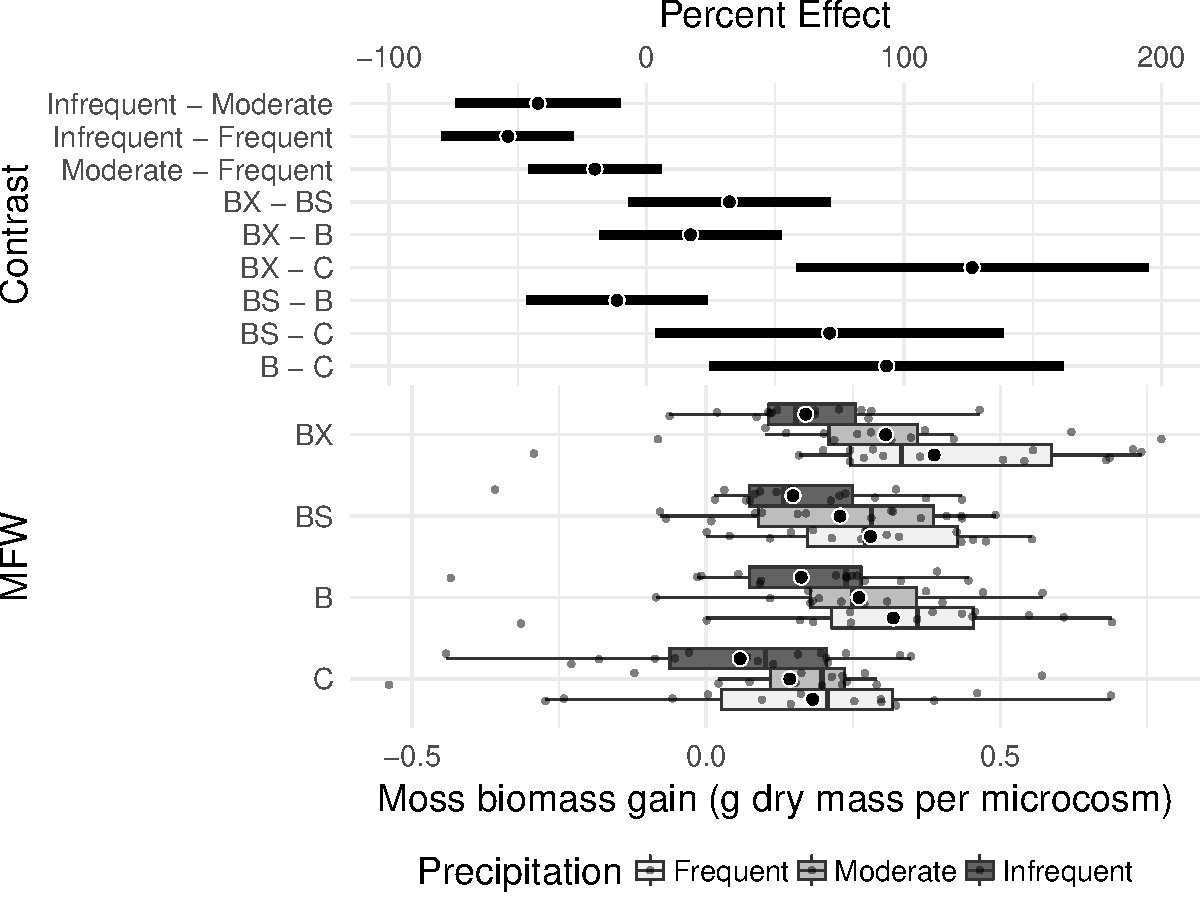
\includegraphics[width=0.9\linewidth]{../output/moss_Hplot} \caption{Harrell plot of moss linear model results. Error bars are 95\% confidence intervals}\label{fig:mossHarrell}
\end{figure}

In figure \ref{fig:mossBar}, I have redrawn figure 3 from Kardol et al.
(2016), which shows treatment means and standard errors for moss biomass
in response to different combinations of community complexity and
precipitation (the original data are available at
\url{https://doi.org/10.5061/dryad.66d5f}). The letters, which indicate
statistically significant \(p\)-values for tests of marginal means
(pooled across the levels of the other factor), draw the researcher and
reader into comparing means using the heights of the bars. The letters
are helpful for this because the standard error bars are not especially
helpful given the computations necessary to go from the illustrated SEMs
to the relevant SEDs.

A major advantage of a Harrell plot (figure \ref{fig:mossHarrell} over
mean-and-error plots with letters or asterisks is that a Harrell plot
nudges researchers to focus on modeled effect size and uncertainty
instead of classification of results into ``significant'' and
``non-significant'' bins. Here, I've scaled the contrasts as percents,
since the units of per microcosm are rather arbitrary. Certainly, one
can use the 95\% confidence limits to mentally bin comparisons into
significant and non-significant bins, but the plot itself does not
encourage it. Instead, the plot encourages a researcher/reader to
consider how the range of values in a CI support, or fail to support,
different interpretations of the results. For example, trivial to
moderate (50\%) reductions in biomass as rain decreases is consistent
with the \(Moderate - Frequent\) contrast CI, but trivial to moderate
increases in biomass as rain decreases are not consistent with the CI.
Means with standard errors supplemented with letters or asterisks do not
convey this information. A bar plot has other disadvanatages relative to
a Harrell plot for these data. For example, the bar plot suggests that
the response (moss biomass gain) is a count, or some other variable that
can only take positive values but the box/dot plot in the bottom panel
of the Harrell plot clearly indicates that moss biomass gain can take
negative values.

\begin{figure}
\includegraphics[width=1\linewidth]{harrell_plot_intro_files/figure-latex/mouseBarPlot-1} \caption{Increase in body fat in the fake mouse data. (A) Percent increase. (B) Raw measures of body fat at baseline and at the end of the treatment period. Error bars are 1SE. }\label{fig:mouseBarPlot}
\end{figure}

\subsection*{Harrell plots explicitly show modeled treatment effects and
uncertainty}\label{harrell-plots-explicitly-show-modeled-treatment-effects-and-uncertainty}
\addcontentsline{toc}{subsection}{Harrell plots explicitly show modeled
treatment effects and uncertainty}

A second major advantage of a Harrell plot over bar plots and Cleveland
dot plots is the explicit, instead of implicit, illustration of modeled
effects and uncertainty, which makes inference from a plot consistent
with inference from a statistical analysis summarized in a table or in
the text. For example, Turnbaugh et al. (2006) published a figure like
that in figure \ref{fig:mouseBarPlot}A, which compares the percent
increase in body fat for mice colonized with microbes from feces from
obese (\emph{ob/ob}) mice and for mice colonized with microbes from
feces from normal (+/+) mice. The data are simulated to mimic the
summary statistics of those given in the original paper (Turnbaugh et
al. 2006; see Walker 2018). Turnbaugh et al. inferred an effect from a
simple \(t\)-test of these percent change scores. The relevant
statistics are the difference in means and the standard error of this
difference (SED). While it is easy to mentally reconstruct the
difference in means from the bar plot, it is very hard to mentally
reconstruct a very useful SED because it is a function of two standard
errors of the mean (SEM) and because both SEMs are noticeably different
for these data. The relevant effect and its error are even harder to
infer from the plot of the raw pre-post means (figure
\ref{fig:mouseBarPlot}B), because the effect is the
\(Time \times Treatment\) interaction.

\begin{figure}
\includegraphics[width=0.7\linewidth]{harrell_plot_intro_files/figure-latex/mouseHarrellPlot-1} \caption{A Harrell plot of the simulated mouse data. Effects are shown as a percent to be consistent with the original plot from Turnbaugh et al. 2006. The lower panel is a box plot of the percent change in body fat weights. The means are shown with the large dot with a white halo. The unconditional difference between these means is 22\%, similar to that in the original data. The upper panel is the contrast between treatment levels -- the difference in percent weight change -- from the linear model with initial weight as a covariate. The error bar is a 95\% confidence interval of this effect. This conditional effect is 3\% and the confidence interval is consistent with both small negative and small positive effects.}\label{fig:mouseHarrellPlot}
\end{figure}

Inference of treatment effect in both analyses in figure
(\ref{fig:mouseBarPlot}A) (which would be the same if the analysis in A
were on the raw change) suffer from regression to the mean (Walker
2018). To avoid this, a linear model including the initial body fat
measure as a covariate should be used. The treatment effect is now
conditional on the initial measure. Unfortunately, it is effectively
impossible to mentally reconstruct a conditional effect like this from
any plot of the raw (unconditional) means, regardless if using a bar
plot, or a dot plot, or a box plot with superimposed means.

By combining a box/dot plot of the raw data and a forest plot of the
modeled effect (figure \ref{fig:mouseHarrellPlot}, a Harrell plot shows
both the raw data and distribution summary and a direct visualization of
the estimated effect and uncertainty. The mouse data are particularly
striking to demonstrate this because of the big difference between the
direct inference from the upper panel and the indirect inference using
the unconditional means in the bottom panel.

\section*{Acknowledgments}\label{acknowledgments}
\addcontentsline{toc}{section}{Acknowledgments}

I want to give huge thanks to the the open source and especially R and R
Studio communities for making easy to implement tools for researchers
and educators.

\newpage

\section*{References}\label{references}
\addcontentsline{toc}{section}{References}

\hypertarget{refs}{}
\hypertarget{ref-Amrhein_earth_2017b}{}
Amrhein, Valentin, Fränzi Korner-Nievergelt, and Tobias Roth. 2017.
``The Earth Is Flat (P~\(>\)~0.05): Significance Thresholds and the
Crisis of Unreplicable Research.'' \emph{PeerJ} 5 (July).
doi:\href{https://doi.org/10.7717/peerj.3544}{10.7717/peerj.3544}.

\hypertarget{ref-Barker_Inference_2008}{}
Barker, Richard J., and Matthew R. Schofield. 2008. ``Inference About
Magnitudes of Effects.'' \emph{International Journal of Sports
Physiology and Performance} 3 (4): 547--57.

\hypertarget{ref-Batterham_Making_2006}{}
Batterham, Alan M., and William G. Hopkins. 2006. ``Making Meaningful
Inferences About Magnitudes.'' \emph{International Journal of Sports
Physiology and Performance} 1 (1): 50--57.

\hypertarget{ref-Curran-Everett_Fundamental_1998}{}
Curran-Everett, Douglas, Sue Taylor, and Karen Kafadar. 1998.
``Fundamental Concepts in Statistics: Elucidation and Illustration.''
\emph{Journal of Applied Physiology} 85 (3): 775--86.

\hypertarget{ref-Drummond_Show_2011}{}
Drummond, G. B., and S. L. Vowler. 2011. ``Show the Data, Don't Conceal
Them.'' \emph{The Journal of Physiology} 589 (8): 1861--3.
doi:\href{https://doi.org/10.1113/jphysiol.2011.205062}{10.1113/jphysiol.2011.205062}.

\hypertarget{ref-Gelman_Values_2013}{}
Gelman, Andrew. 2013. ``P Values and Statistical Practice:''
\emph{Epidemiology} 24 (1): 69--72.
doi:\href{https://doi.org/10.1097/EDE.0b013e31827886f7}{10.1097/EDE.0b013e31827886f7}.

\hypertarget{ref-Greenland_Living_2013}{}
Greenland, Sander, and Charles Poole. 2013. ``Living with P Values.''
\emph{Epidemiology} 24 (1): 62--68.
doi:\href{https://doi.org/10.1097/EDE.0b013e3182785741}{10.1097/EDE.0b013e3182785741}.

\hypertarget{ref-Harrell_Principles_2014}{}
Harrell, Frank E. 2014. ``Principles of Graph Construction.''

\hypertarget{ref-Johnson_insignificance_1999}{}
Johnson, Douglas H. 1999. ``The Insignificance of Statistical
Significance Testing.'' \emph{The Journal of Wildlife Management},
763--72.

\hypertarget{ref-KaelinJr_Publish_2017}{}
Kaelin Jr, William G. 2017. ``Publish Houses of Brick, Not Mansions of
Straw.'' \emph{Nature News} 545 (7655): 387.
doi:\href{https://doi.org/10.1038/545387a}{10.1038/545387a}.

\hypertarget{ref-Kardol_Trophic_2016}{}
Kardol, Paul, Clydecia M. Spitzer, Michael J. Gundale, Marie-Charlotte
Nilsson, and David A. Wardle. 2016. ``Trophic Cascades in the
Bryosphere: The Impact of Global Change Factors on Top-down Control of
Cyanobacterial N \textsubscript{2} -Fixation.'' Edited by Mark Gessner.
\emph{Ecology Letters} 19 (8): 967--76.
doi:\href{https://doi.org/10.1111/ele.12635}{10.1111/ele.12635}.

\hypertarget{ref-Krzywinski_Points_2014}{}
Krzywinski, Martin, and Naomi Altman. 2014. ``Points of Significance:
Visualizing Samples with Box Plots.'' \emph{Nature Methods} 11 (2):
119--20.

\hypertarget{ref-Munafo_Robust_2018}{}
Munafò, Marcus R., and George Davey Smith. 2018. ``Robust Research Needs
Many Lines of Evidence.'' News. \emph{Nature}.
http://www.nature.com/articles/d41586-018-01023-3.
doi:\href{https://doi.org/10.1038/d41586-018-01023-3}{10.1038/d41586-018-01023-3}.

\hypertarget{ref-Nakagawa_Effect_2007}{}
Nakagawa, S, and I C Cuthill. 2007. ``Effect Size, Confidence Interval
and Statistical Significance: A Practical Guide for Biologists.''
\emph{Biological Reviews}, January, 591--605.
doi:\href{https://doi.org/10.1111/j.1469-185x.2007.00027.x}{10.1111/j.1469-185x.2007.00027.x}.

\hypertarget{ref-Rousselet_few_2016}{}
Rousselet, Guillaume A., John J. Foxe, and J. Paul Bolam. 2016. ``A Few
Simple Steps to Improve the Description of Group Results in
Neuroscience.'' \emph{European Journal of Neuroscience} 44 (9):
2647--51.
doi:\href{https://doi.org/10.1111/ejn.13400}{10.1111/ejn.13400}.

\hypertarget{ref-Spitzer_BoxPlotR_2014}{}
Spitzer, Michaela, Jan Wildenhain, Juri Rappsilber, and Mike Tyers.
2014. ``BoxPlotR: A Web Tool for Generation of Box Plots.'' \emph{Nature
Methods} 11 (2): 121--22.

\hypertarget{ref-Tukey_Philosophy_1991}{}
Tukey, John W. 1991. ``The Philosophy of Multiple Comparisons.''
\emph{Statistical Science} 6 (1): 100--116.

\hypertarget{ref-Turnbaugh_obesityassociated_2006a}{}
Turnbaugh, Peter J., Ruth E. Ley, Michael A. Mahowald, Vincent Magrini,
Elaine R. Mardis, and Jeffrey I. Gordon. 2006. ``An Obesity-Associated
Gut Microbiome with Increased Capacity for Energy Harvest.''
\emph{Nature} 444 (7122): 1027--31.
doi:\href{https://doi.org/10.1038/nature05414}{10.1038/nature05414}.

\hypertarget{ref-Vaux_Research_2012}{}
Vaux, David L. 2012. ``Research Methods: Know When Your Numbers Are
Significant.'' \emph{Nature} 492 (7428): 180--81.
doi:\href{https://doi.org/10.1038/492180a}{10.1038/492180a}.

\hypertarget{ref-Walker_Bias_2018}{}
Walker, Jeffrey A. 2018. ``Bias in Pre-Post Designs - an Example from
the Turnbaugh et Al (2006) Mouse Fecal Transplant Study.''
\emph{Https://Www.middleprofessor.com/Files/Quasipubs/Change\_scores.html},
March.
doi:\href{https://doi.org/10.6084/m9.figshare.6025571}{10.6084/m9.figshare.6025571}.

\hypertarget{ref-Weissgerber_Transparent_2016}{}
Weissgerber, Tracey L, Vesna D Garovic, Stacey J Winham, Natasa M Milic,
and Eric M Prager. 2016. ``Transparent Reporting for Reproducible
Science.'' \emph{Journal of Neuroscience Research} 94 (10): 859--64.
doi:\href{https://doi.org/10.1002/jnr.23785}{10.1002/jnr.23785}.

\hypertarget{ref-Weissgerber_Bar_2015}{}
Weissgerber, Tracey L., Natasa M. Milic, Stacey J. Winham, and Vesna D.
Garovic. 2015. ``Beyond Bar and Line Graphs: Time for a New Data
Presentation Paradigm.'' \emph{PLOS Biology} 13 (4): e1002128.
doi:\href{https://doi.org/10.1371/journal.pbio.1002128}{10.1371/journal.pbio.1002128}.

\hypertarget{ref-Yoccoz_Use_1991}{}
Yoccoz, Nigel G. 1991. ``Use, Overuse, and Misuse of Significance Tests
in Evolutionary Biology and Ecology.'' \emph{Bulletin of the Ecological
Society of America} 72 (2): 106--11.



\end{document}
